\iffalse
\title{}
\author{EE24BTECH11053 - S A Aravind Eswar}
\chapter{2007}
\section{ae}
\fi
    \item $\lim_{x\to 0}\frac{\sin x}{e^x x}$\hfill{[2007-AE]}
        \begin{enumerate}
                \begin{multicols}{4}
            \item 10
            \item 0
            \item 1
            \item $\infty$
                \end{multicols}
        \end{enumerate}
    \item Let a dynamical system be described by the differential equation $\displaystyle2\frac{dx}{dx} + \cos x = 0$. Which of the following differential equations describes this system in a close approximation sense for small perturbation around $x = \pi / 4$?\hfill{[2007-AE]}
        \begin{enumerate}
                \begin{multicols}{2}
            \item $s\frac{dx}{dt}+\sin x = 0$
            \item $2\frac{dx}{dt} - \frac{1}{\sqrt{2}}x=0$
            \item $\frac{dx}{dt}+ \cos x = 0$
            \item $\frac{dx}{dt} + x = 0$
                \end{multicols}
        \end{enumerate}

        \textbf{Common Data for Questions \ref{itm:71}, \ref{itm:72} \& \ref{itm:73}:} An Airplane designer what to keep longitudnal static stability margin($SM$)  within 5\% to 15\% of mean aerodynamic chord. A wind tunnel test of the model showed that for $\displaystyle\bar{X}_CG = 0.3, \frac{dC_m}{dC_\perp} = 0.1$. Note that the distance from the wing leading edge to the center of gravity ($X_CG$) has been non-dimentionalizes by dividing it with mean aerodynamic chord, $\bar{c}$, such that $\bar{X}_CG = X_CG/\bar{c}$. Note also that the relation $\displaystyle\frac{dC_m}{dC_\perp} = -SM$ holds true for this airplane.
    \item The most forward location of the airplane center of gravity permitted to fulfill the designer's requirement on longitudinal static margin is \label{itm:71}\hfill{[2007-AE]}
        \begin{enumerate}
                \begin{multicols}{4}
            \item $0.35 \bar{c}$
            \item $0.25 \bar{c}$
            \item $0.15 \bar{c}$
            \item $0.52 \bar{c}$
                \end{multicols}
        \end{enumerate}
    \item The most aft location of the airplane centere of the gravity permitted to fulfill designer's requirement of longitudnal static stability is\label{itm:72}\hfill{[2007-AE]}
        \begin{enumerate}
                \begin{multicols}{4}
            \item $0.35 \bar{c}$
            \item $0.45 \bar{c}$
            \item $0.52 \bar{c}$
            \item $0.67 \bar{c}$
                \end{multicols}
        \end{enumerate}
    \item The center of gravity location to have $\displaystyle\frac{d\delta e}{dC_L}=0$\label{itm:73}\hfill{[2007-AE]}
        \begin{enumerate}
                \begin{multicols}{4}
            \item $0.35 \bar{c}$
            \item $0.45 \bar{c}$
            \item $0.5 \bar{c}$
            \item $0.4 \bar{c}$
                \end{multicols}
        \end{enumerate}

        \textbf{Common Data for Questions \ref{itm:74} \& \ref{itm:75}:} Consider the spring mass system shown in the figure below. This system has two degrees of freedom representing ther motions of the two masses.

\begin{figure}
    
    \begin{tikzpicture}

% Define parameters
\def\zigzag{0.15} % Height of zigzag spring
\def\springlen{1.5} % Length of each spring segment
\def\masswidth{1}   % Width of the mass box
\def\massheight{1}  % Height of the mass box
\def\wheelradius{0.15} % Radius of the wheels


% Function to draw a zigzag spring
\newcommand{\drawzigzagspring}[2]{
  \foreach \i in {0,1,...,5}
  {
    \draw[thick] (#1+\i*\springlen/6,0.75+\zigzag) -- ++(\springlen/12,-2*\zigzag) -- ++(\springlen/12,2*\zigzag);
  }
}

% Ground line
\draw[thick] (0,0.05) -- (2,0.05);

\draw[thick] (2.5,0.05) -- (4.5,0.05);
% Left wall
\draw[thick] (-1,0) -- (-1,1.5);

% Left spring
\drawzigzagspring{-1}{0.5}

% Left mass (mass m)
\draw[thick] (0.5,0.25) rectangle ++(\masswidth,\massheight);
\node at (1,0.75) {$m$};

% Middle spring
\drawzigzagspring{1.5}{3}

% Right mass (mass 3m)
\draw[thick] (3,0.25) rectangle ++(\masswidth,\massheight);
\node at (3.5,0.75) {$3m$};

% Right spring
\drawzigzagspring{4}{5.5}

% Right wall
\draw[thick] (5.5,0) -- (5.5,1.5);

% Labels
\node at (-0.25,1.25) {$k$};
\node at (2.25,1.25) {$k$};
\node at (4.75,1.25) {$k$};

% Arrows for x1 and x2
\draw[->] (1,1.5) -- ++(0.5,0) node[right] {$x_1$};
\draw[->] (3.5,1.5) -- ++(0.5,0) node[right] {$x_2$};

\fill (3.25,0.25) circle (\wheelradius);
\fill (3.75,0.25) circle (\wheelradius);

% Left mass wheels
\fill (0.75,0.25) circle (\wheelradius);
\fill (1.25,0.25) circle (\wheelradius);

\end{tikzpicture}


        
\end{figure}
    
    \item The system shows the following type of coordination coupling \label{itm:74}\hfill{[2007-AE]}
        \begin{enumerate}
            \item static coupling
            \item dynamic coupling
            \item static and dynamic coupling
            \item no coupling
        \end{enumerate}
    \item The two natural frequencies of the system are given as\label{itm:75}\hfill{[2007-AE]}
        \begin{enumerate}
                \begin{multicols}{2}
            \item $\displaystyle\sqrt{\frac{4\pm\sqrt{5}}{3}\frac{k}{m}}$
            \item $\displaystyle\sqrt{\frac{4\pm\sqrt{3}}{3}\frac{k}{m}}$
            \item $\displaystyle\sqrt{\frac{4\pm\sqrt{7}}{3}\frac{k}{m}}$
            \item $\displaystyle\sqrt{\frac{4\pm\sqrt{11}}{3}\frac{k}{m}}$
                \end{multicols}
        \end{enumerate}

\textbf{Statement for Linked Answer Question \ref{itm:76} \& \ref{itm:77}:} For a piston propeller airplane weighing 20000 N, the flight testing at 5 km pressure alitude in standard atmosphere gave the variation of power required versus true are speed as showen in the figure below. The student forgot to label the air speed axis. The maximum climb rate at sea was calculated to be 4m/s. assume shaft power available to be independent of speed of flight. For piston propellow airplane, it can be assumed that the shaft power available is propotional to ambient density. Values of air density at sea level and at 5 km pressure altitude are 1.225 kg/m$^3$ and 0.74 kg/m$^3$ respectively.

        \begin{figure}
            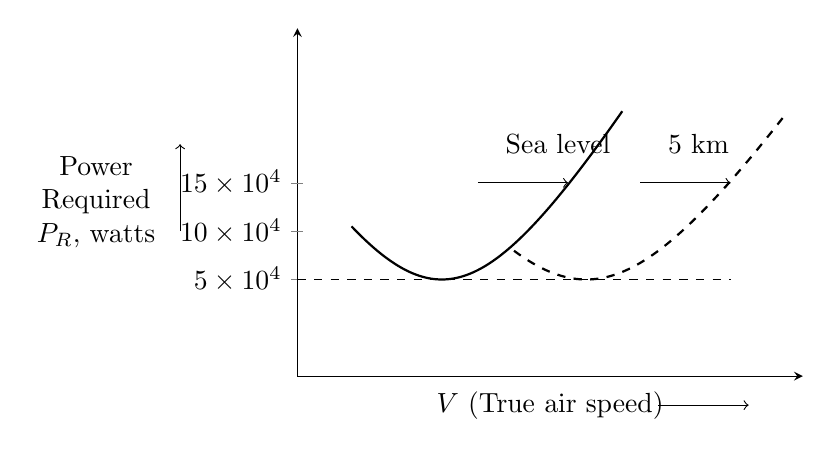
\begin{tikzpicture}
    \begin{axis}[
        width=8cm, height=6cm, % Adjusted size for a more compact graph
        xmin=0, xmax=1.4,
        ymin=0, ymax=1.8,
        axis lines=left,
        xlabel={$V$ (True air speed)},
        ylabel={Power\\Required\\$P_R$, watts},
        ylabel style={rotate=-90, align=center},
        xtick=\empty, ytick=\empty,
        extra y ticks={0.5, 0.75, 1},
        extra y tick labels={$5 \times 10^4$, $10 \times 10^4$, $15 \times 10^4$},
        extra x ticks={},
        clip=false
    ]
    
    % Sea level curve (solid line with dip)
    \addplot[
        domain=0.15:0.9,
        samples=100,
        thick
    ]
    {(1+(10*(x-0.4)^2))^(0.5)-0.5}; % Adjusted formula for a more pronounced dip and rise
    \node[right] at (axis cs:0.55,1.2) {Sea level};
    
\draw[->] (0.5,1) -- ++(0.25,0) node[right] {};
\draw[->] (0.95,1) -- ++(0.25,0) node[right] {};
\draw[->] (1,-0.15) -- ++(0.25,0) node[right] {};
\draw[->] (-0.325,0.75) -- ++(0,0.45) node[right]{} ;
    % 5 km curve (dashed line with similar shape but slightly higher)
    \addplot[
        domain=0.6:1.35,
        samples=100,
        thick,
        dashed
    ]
    {(1+(8*(x-0.8)^2))^(0.5)-0.5}; % Adjusted formula for 5 km
    \node[right] at (axis cs:1,1.2) {5 km};

    % Dashed horizontal line at y=0.5
    \draw[dashed] (axis cs:0,0.5) -- (axis cs:1.2,0.5);

    \end{axis}
\end{tikzpicture}


        \end{figure}

    \item The maximum rate of climb achieved by this airplane at 5 km altitude will be\label{itm:76}\\\strut\hfill{[2007 - AE]}
        \begin{enumerate}
                \begin{multicols}{4}
            \item 1.65 m/s
            \item 0.51 m/s
            \item 1.43 m/s
            \item 3.65 m/s
                \end{multicols}
        \end{enumerate}
    \item If during the maximum rate of climb at 5 km altitude, the airplane was flying at an angle of attack of 4 degrees and altitude (pitch) angle of 5 degrees, what was the equivalent airspeed of the airplane?\label{itm:77}\hfill{[2007-AE]}
        \begin{enumerate}
                \begin{multicols}{4}
            \item 40.2 m/s
            \item 63.7 m/s
            \item 130.3 m/s
            \item 20.2 m/s
                \end{multicols}
        \end{enumerate}

\textbf{Statement for Linked Answer Questions \ref{itm:78} \& \ref{itm:79}:} A modal winf rectangular platform has a chort 0.2m and a span 1.2m. It has a symmetric airfoil section whose lift curve slope is 0.1 per degree. When this wing is mounted at 8 degrees angle of attack in a freestream of 20 m/s it is found to develop 35.3N lift when the density of air 1.225 kg/m$^3$.

    \item The lift curve slope of this wing is\label{itm:78}\hfill{[2007-AE]}
        \begin{enumerate}
                \begin{multicols}{4}
            \item 0.10 per deg
            \item 0.092 per deg
            \item 0.075 per deg
            \item 0.050 per deg
                \end{multicols}
        \end{enumerate}
    \item The pan efficiency factor of this wing is\label{itm:79}\hfill{[2007-AE]}
        \begin{enumerate}
                \begin{multicols}{4}
            \item 1.0
            \item 0.91
            \item 0.75
            \item 0.63
                \end{multicols}
        \end{enumerate}

\textbf{Statement for Linked Answer Question \ref{itm:80} \& \ref{itm:81}:}

Let $$F(s) = \frac{\brak{s+10}}{\brak{s+2}\brak{s+20}}$$

    \item the partial fraction expression of $F(s)$\label{itm:80}\hfill{[2007-AE]}
        \begin{enumerate}
                \begin{multicols}{2}
            \item $\displaystyle\frac{1}{s+2}+\frac{1}{s+20}$
            \item $\displaystyle\frac{5}{s+2}+\frac{2}{s+20}$
            \item $\displaystyle\frac{2}{s+2}+\frac{20}{s+20}$
            \item $\displaystyle\frac{4/9}{s+2}+\frac{5/9}{s+20}$
                \end{multicols}
        \end{enumerate}
    \item The inverse Laplace transform of $F(s) is$\label{itm:81}\hfill{[2007-AE]}
        \begin{enumerate}
                \begin{multicols}{2}
            \item $\displaystyle 2e^{-2s}+20e^{-20s}$
            \item $\displaystyle\frac{4}{9}e^{2s}+\frac{5}{9}e^{-20s}$
            \item $5e^{-2s}+2e^{-20s}$
            \item $\frac{9}{4}e^{-2s}+\frac{9}{5}e^{-20s}$
                \end{multicols}
        \end{enumerate}

\textbf{Statement for Linked Answer Questions \ref{itm:82} \& \ref{itm:83}: }The equation of motion of a vibrating rod is given by $\frac{\partial^2u}{\partial x^2} = \frac{1}{c^2}\frac{\partial^2u}{\partial x^2}$. Here $u$ is the displacmet along the rod and is a function of both position $x$ and the time $t$. To find the response of the vibrating rod, we need to solve this equation using boundary conditions and initial conditions.

    \item The Boundary conditions needed for a rod fixed at the root ($x=0$) and free at the tip ($x=l$) are\label{itm:82}\hfill{[2007-AE]}
  \begin{enumerate}
          \begin{multicols}{2}
      \item $u(x=0)=0,\frac{\partial u}{\partial x}(x=l)=0$
      \item $u(x=l)=0,\frac{\partial u}{\partial x}(x=l)=0$
    \item $u(x=l)=0,u(x=l)=0$
    \item $\frac{\partial u}{\partial x}(x=0)=0, \frac{\partial u}{\partial x}(x=l)=0$
          \end{multicols}
  \end{enumerate}
  \item If the polytropic efficiency of the compressor is 0.89, then the isentropic efficiency of the compressor is\label{itm:83}\hfill{[2007-AE]}
  \begin{enumerate}
          \begin{multicols}{4}
      \item $\cos(\frac{\omega l}{c})=0$
      \item $\sin (\frac{\omega l}{c})=0$
      \item $\cos (\frac{\omega c}{l})=0$
      \item $\cos (\frac{\omega}{c})=0$
          \end{multicols}
  \end{enumerate}



\textbf{Statement for Linked Answer Questions \ref{itm:84} \& \ref{itm:85}:} Air enters the compressor of a gas turbine engine with velocity 127 m/s, density 1.2 kg/m$^3$ and stagnation pressure 0.9 MPa. Air exits the compressor with velocity 139 m/s and stagnation pressure 3.15 MPa. Assume that the ratio of specific heats is constant and equal to 1.4.
  \item The compressor pressure ratio is\label{itm:84}\hfill{[2007-AE]}
  \begin{enumerate}
          \begin{multicols}{4}
    \item 0.22
    \item 0.28
    \item 3.50
    \item 3.90
          \end{multicols}
  \end{enumerate}
  \item If the polytropic efficiency of the compressor is 0.89, then the isentropic efficiency of the compressor is\label{itm:85}\hfill{[2007-AE]}
  \begin{enumerate}
          \begin{multicols}{4}
    \item 0.613
    \item 0.869
    \item 0.89
    \item 0.98
          \end{multicols}
  \end{enumerate}


